\chapter*{Badania}

Celem tego rozdziału jest przeprowadzenie analizy wyników klasyfikacji obrazów zwierząt dla modeli ResNet i 
ConvNeXt. Analiza obejmuje porównanie skuteczności modeli w różnych scenariuszach modyfikacji tła oraz w zależności 
od wielkości obiektu na obrazie. Przeanalizowane zostaną ogólne metryki, wyniki dla poszczególnych klas oraz wpływ 
wielkości obiektu na dokładność klasyfikacji.

\section*{Wyniki ogólne}

Badania miały na celu zbadanie wpływu modyfikacji tła na skuteczność klasyfikacji obrazów za pomocą dwóch modeli głębokiego uczenia: ResNet 
oraz ConvNeXt. W tym celu dokonano obliczeń podstawowych metryk, takich jak Accuracy, Precision, Recall i F1-score, dla oryginalnych oraz 
zmodyfikowanych obrazów, traktując wszystkie modyfikację jako jedną grupę.

Dla modelu ResNet, na oryginalnych obrazach uzyskano Accuracy na poziomie 0.886500, Precision 0.967026, Recall 0.886500 i F1-score 0.922742. 
Po modyfikacji tła wartości te uległy znacznemu obniżeniu, osiągając odpowiednio 0.697018 dla Accuracy, 0.948539 dla Precision, 0.697018 dla 
Recall i 0.802350 dla F1-score. W przypadku modelu ConvNeXt, na oryginalnych obrazach uzyskano wartości: Accuracy 0.943300, Precision 0.972519, 
Recall 0.943300 i F1-score 0.956791. Podobnie jak w przypadku ResNet, modyfikacja tła spowodowała obniżenie tych wartości, osiągając 
Accuracy 0.790873, Precision 0.961080, Recall 0.790873 i F1-score 0.866282.

Analiza wyników wskazuje, że modyfikacja tła negatywnie wpływa na skuteczność obu modeli, jednak model ConvNeXt wykazuje większą odporność na 
zmiany tła niż ResNet. Model ConvNeXt osiąga wyższe wartości metryk zarówno dla oryginalnych, jak i zmodyfikowanych obrazów, co sugeruje jego 
większą stabilność i lepszą adaptację do różnych warunków. Wartości metryk dla zmodyfikowanych obrazów są niższe w przypadku ResNet, co może 
wskazywać na większą wrażliwość tego modelu na zmiany w tle.

Wnioski z badań sugerują, że dla zadań klasyfikacyjnych, gdzie modyfikacje tła mogą występować, model ConvNeXt jest bardziej odpowiedni. 
Dalsze badania nad metodami przetwarzania i augmentacji danych mogą pomóc w zminimalizowaniu wpływu modyfikacji tła na wyniki klasyfikacji, 
co jest kluczowe dla poprawy dokładności i niezawodności modeli głębokiego uczenia. Wyniki te podkreślają znaczenie wyboru odpowiedniego 
modelu oraz technik przetwarzania danych w kontekście zadań związanych z klasyfikacją obrazów.

\begin{table}
	\centering
	\begin{tabular}{|c|c|c|c|c|c|}
		\hline
		\textbf{Model} & \textbf{Type} & \textbf{Accuracy} & \textbf{Precision} & \textbf{Recall} & \textbf{F1-score} \\
		\hline
		ResNet & Original & 0.886500 & 0.967026 & 0.886500 & 0.922742 \\
		\hline
		ResNet & Modified & 0.697018 & 0.948539 & 0.697018 & 0.802350 \\
		\hline
		ConvNeXt & Original & 0.943300 & 0.972519 & 0.943300 & 0.956791 \\
		\hline
		ConvNeXt & Modified & 0.790873 & 0.961080 & 0.790873 & 0.866282 \\
		\hline
	\end{tabular}
	\caption{Metryki porównawcze modeli ResNet i ConvNeXt}
	\label{tab:model_comparison_metrics}
\end{table}

Wyniki badań również wskazują, że pomimo modyfikacji tła, Precision dla obu modeli (ResNet i ConvNeXt) uległa jedynie niewielkiemu spadkowi. 
Dla ResNet Precision zmniejszyła się z 0.967026 na 0.948539, a dla ConvNeXt z 0.972519 na 0.961080. Mały spadek Precision w obu przypadkach 
sugeruje, że oba modele nadal skutecznie identyfikują prawdziwie pozytywne przypadki, nawet po modyfikacji tła.

To zjawisko można interpretować jako wskazówkę, że oba modele są dobrze dostrojone do rozpoznawania właściwych cech istotnych dla klasyfikacji, 
niezależnie od zmieniającego się tła. Wysoka wartość Precision oznacza, że modele rzadko identyfikują fałszywie pozytywne przypadki, co jest 
szczególnie istotne w zastosowaniach, gdzie dokładność klasyfikacji jest kluczowa. Niewielki spadek Precision w przypadku modyfikacji tła 
sugeruje, że modele są w stanie skutecznie ignorować zmiany w tle i skoncentrować się na istotnych cechach obiektów, co jest pozytywnym aspektem 
ich działania.
\begin{figure}
	\centering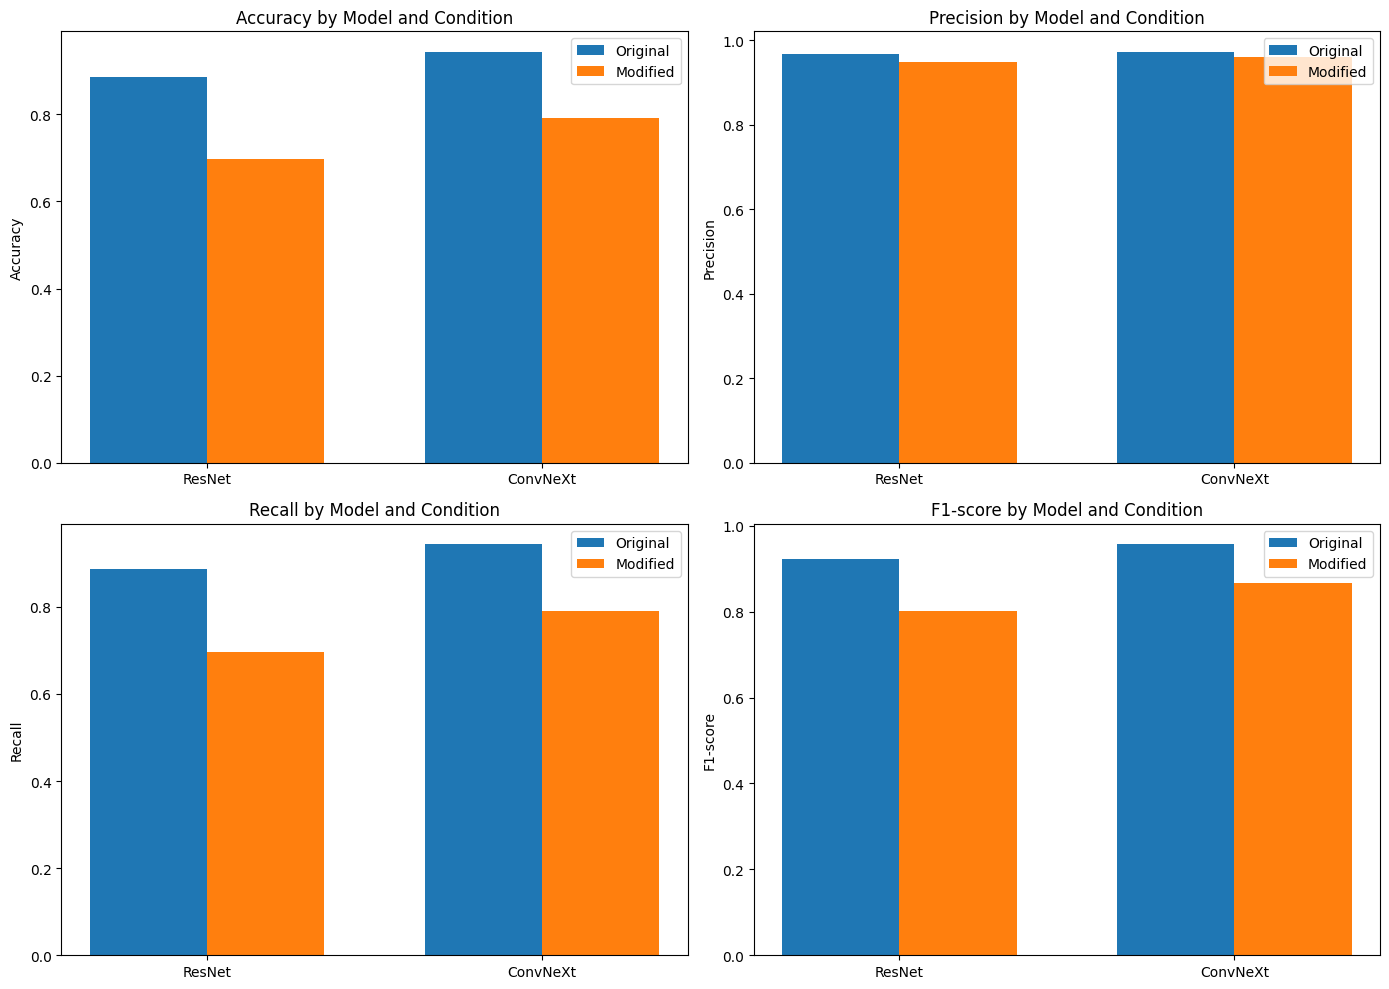
\includegraphics[width=.9\textwidth]{img/overall_metrics}
	\caption{Metryki dla danych oryginalnych zestawionych z danymi o zmodyfikowanych tłach}  
    \label{rys:overall_metrics}
\end{figure}


W badaniach obliczono również średnie wartości confidence scores dla dwóch modeli: ResNet oraz ConvNeXt. Wartości te obejmują ogólną średnią 
confidence score, a także średnie confidence scores dla poprawnych i niepoprawnych klasyfikacji. Dla modelu ResNet na oryginalnych obrazach 
średnia confidence score wyniosła 85.188854, ze średnią wartością 89.137424 dla poprawnych klasyfikacji i 54.348263 dla niepoprawnych. Po 
modyfikacji tła, średnia confidence score spadła do 71.694490, ze średnią wartością 83.929904 dla poprawnych klasyfikacji i 43.546579 dla 
niepoprawnych.

W przypadku modelu ConvNeXt na oryginalnych obrazach średnia confidence score wyniosła 68.527975, ze średnią wartością 70.036361 dla poprawnych 
klasyfikacji i 43.433439 dla niepoprawnych. Po modyfikacji tła, średnia confidence score spadła do 57.543545, ze średnią wartością 63.189640 dla 
poprawnych klasyfikacji i 36.191272 dla niepoprawnych.

Wyniki te wskazują na znaczący spadek średnich confidence scores dla obu modeli po modyfikacji tła. Średnie confidence scores dla poprawnych 
klasyfikacji są wyższe niż dla niepoprawnych w obu przypadkach, co sugeruje, że modele są bardziej pewne swoich poprawnych klasyfikacji. Jednak 
modyfikacja tła powoduje ogólny spadek pewności modeli, co może być wynikiem zmniejszenia jasności sygnałów związanych z obiektami do 
rozpoznania.

Analiza wartości confidence scores dla ConvNeXt wskazuje na większy spadek w porównaniu do ResNet. Model ConvNeXt na oryginalnych obrazach ma 
niższą ogólną średnią confidence score (68.527975) w porównaniu do ResNet (85.188854). Jednakże, spadek ten jest bardziej wyraźny po modyfikacji 
tła, gdzie średnia confidence score dla ConvNeXt wynosi 57.543545, podczas gdy dla ResNet jest to 71.694490.

Podsumowując, modyfikacja tła ma wyraźny wpływ na zmniejszenie pewności klasyfikacji obrazów przez modele ResNet i ConvNeXt. Chociaż oba modele 
wykazują wysoką pewność przy poprawnych klasyfikacjach, modyfikacja tła powoduje ogólny spadek tych wartości, z bardziej zauważalnym spadkiem w 
przypadku modelu ConvNeXt. Wyniki te podkreślają znaczenie zrozumienia i zarządzania wpływem tła na wydajność modeli klasyfikacyjnych w 
praktycznych zastosowaniach.

\begin{table}
	\centering
	\begin{tabular}{|c|c|c|c|c|c|}
		\hline
		\textbf{Model} & \textbf{Type} & \textbf{Average} & 
		\textbf{Average correct} & \textbf{Average incorrect} \\
		\hline
		ResNet & Original & 85.188854 & 89.137424 & 54.348263 \\
		\hline
		ResNet & Modified & 71.694490 & 83.929904 & 43.546579  \\
		\hline
		ConvNeXt & Original & 68.527975 & 70.036361 & 43.433439 \\
		\hline
		ConvNeXt & Modified & 57.543545 & 63.189640 & 36.191272 \\
		\hline
	\end{tabular}
	\caption{Confidence scores dla modeli ResNet i ConvNeXt}
	\label{tab:model_confidence}
\end{table}

\begin{figure}
	\centering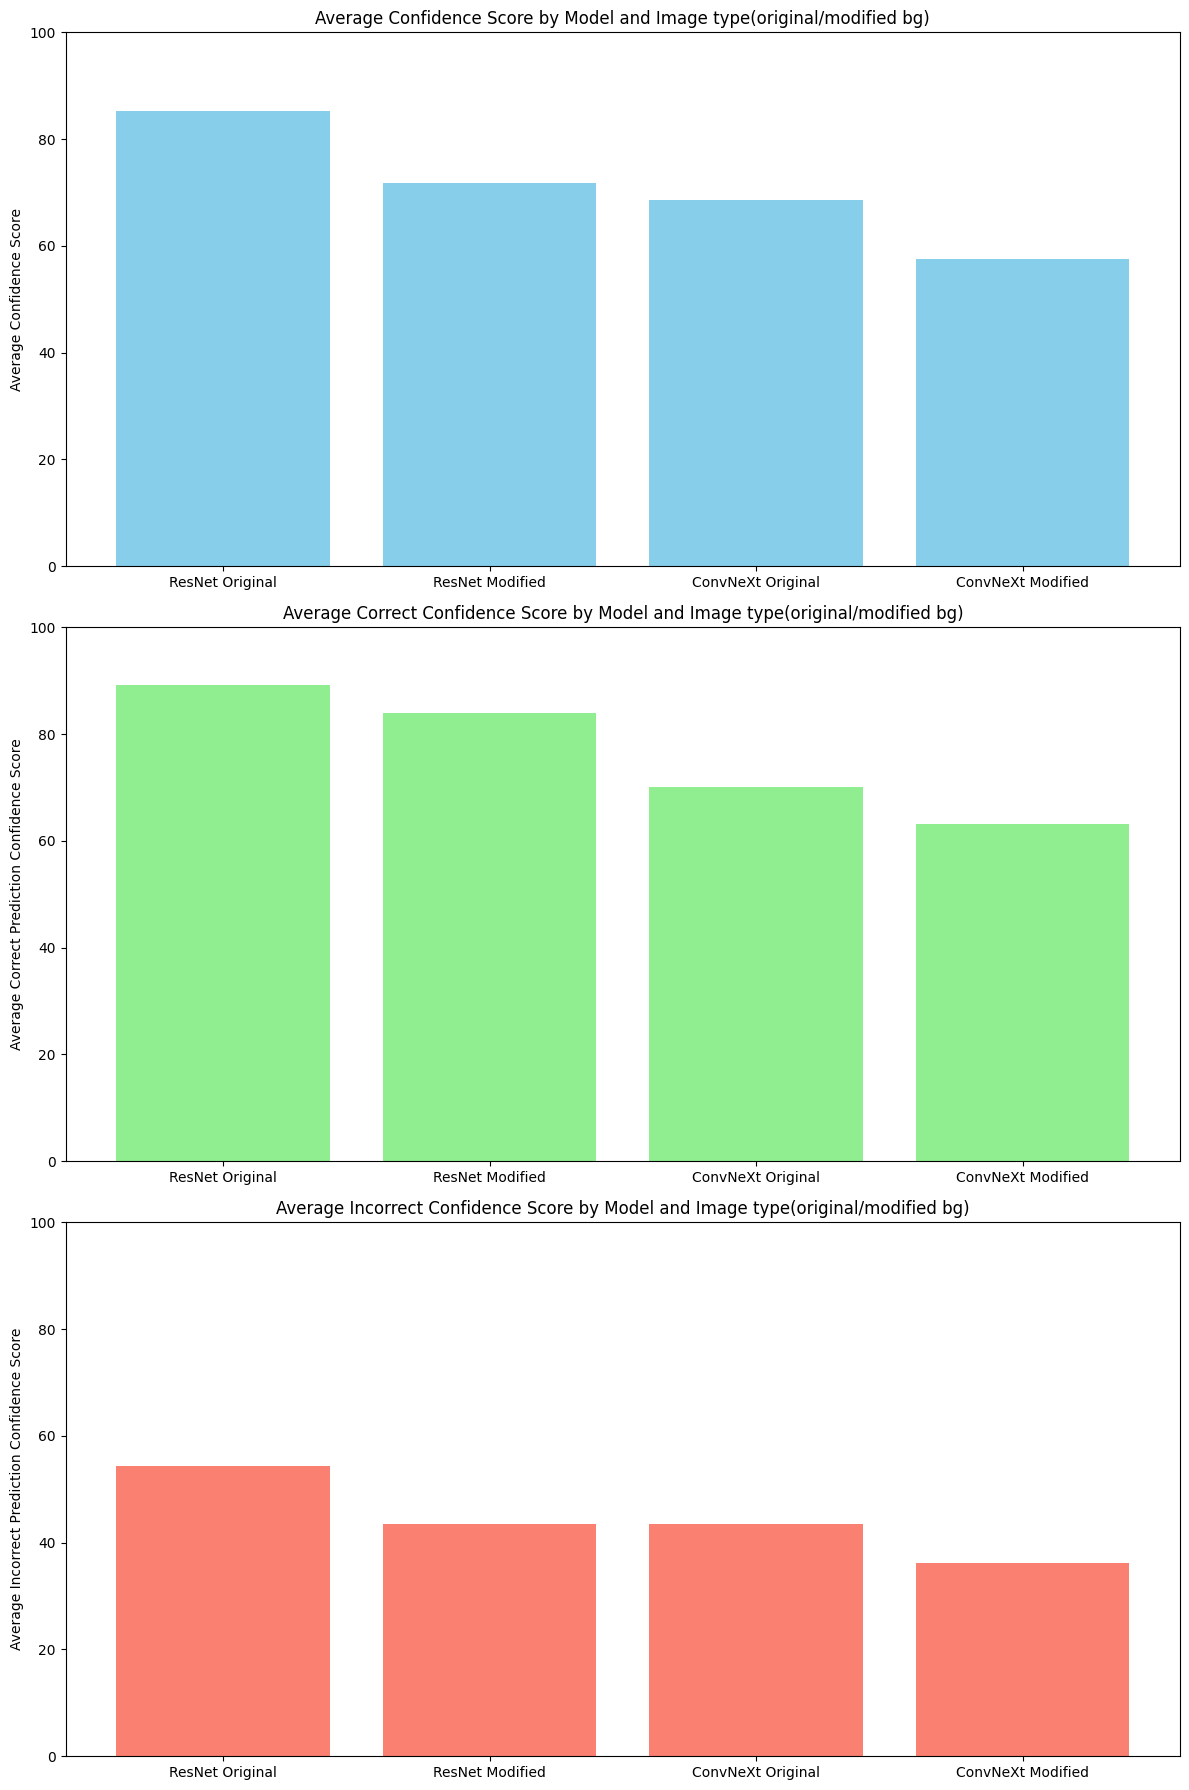
\includegraphics[width=.9\textwidth]{img/confidence_avg}
	\caption{Średnie wartości dla confidence scores}  
    \label{rys:confidence_avg}
\end{figure}
\newpage
Na podstawie dystrybucji confidence scores dla modeli ResNet i ConvNeXt można wyciągnąć kilka istotnych wniosków. Model ResNet wykazuje wysoką 
pewność dla poprawnych klasyfikacji, z koncentracją confidence scores w przedziale od 80 do 100, co wskazuje na jego stabilność w 
identyfikowaniu prawidłowych przypadków. W przypadku błędnych klasyfikacji confidence scores są bardziej równomiernie rozłożone, co oznacza, 
że model jest mniej pewny, gdy się myli. Z kolei model ConvNeXt ma szerszy rozkład confidence scores, z wyraźnym pikiem dla poprawnych 
klasyfikacji w przedziale 70-80 i dla błędnych w przedziale 30-40. Sugeruje to, że ConvNeXt jest mniej pewny swoich poprawnych decyzji w 
porównaniu do ResNet i bardziej skłonny do popełniania błędów z dużą pewnością. Te różnice w rozkładzie pewności klasyfikacji wskazują, że 
ResNet jest bardziej stabilny, podczas gdy ConvNeXt wykazuje większą różnorodność w pewności decyzji, co może wpływać na jego wydajność w 
obliczu modyfikacji tła.

\begin{figure}
	\centering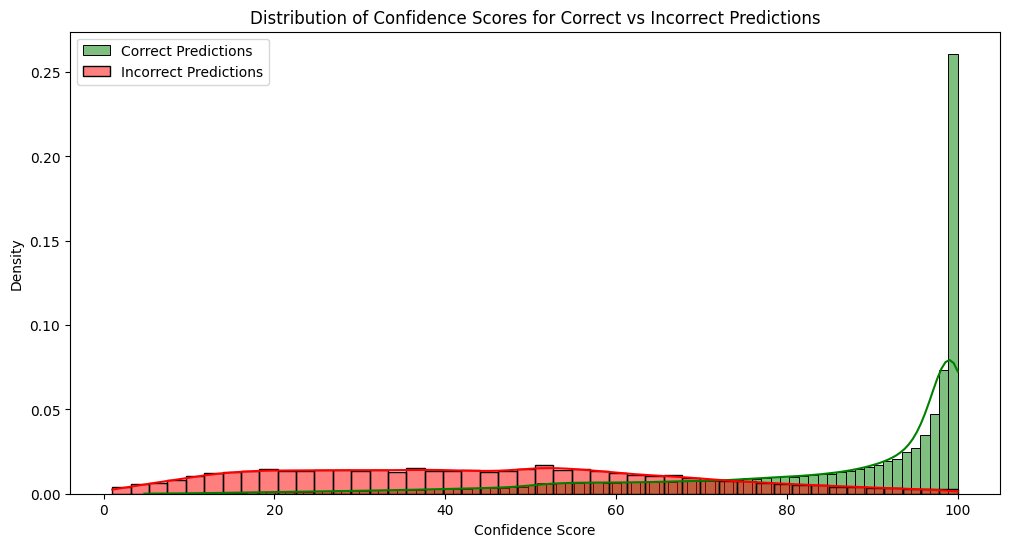
\includegraphics[width=.9\textwidth]{img/resnet_conf_distro}
	\caption{Dystrybucja confidence score dla ResNet}
	\label{rys:res_c_distro}
\end{figure}

\begin{figure}
	\centering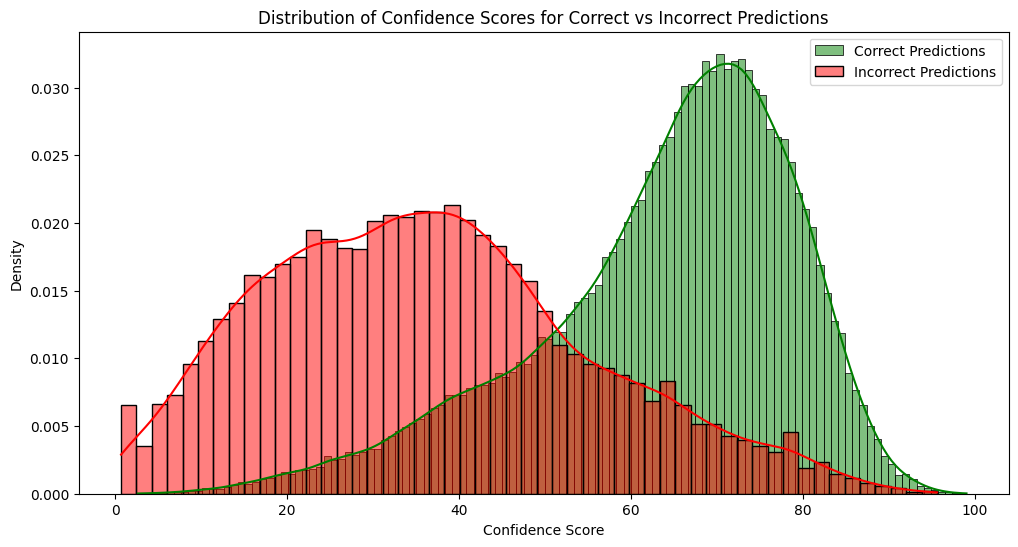
\includegraphics[width=.9\textwidth]{img/convnext_conf_distro}
	\caption{Dystrybucja confidence score dla ConvNext}
	\label{rys:conv_c_distro}
\end{figure}
\newpage
\section*{Wyniki względem kategorii wielkości}


\begin{figure}
	\centering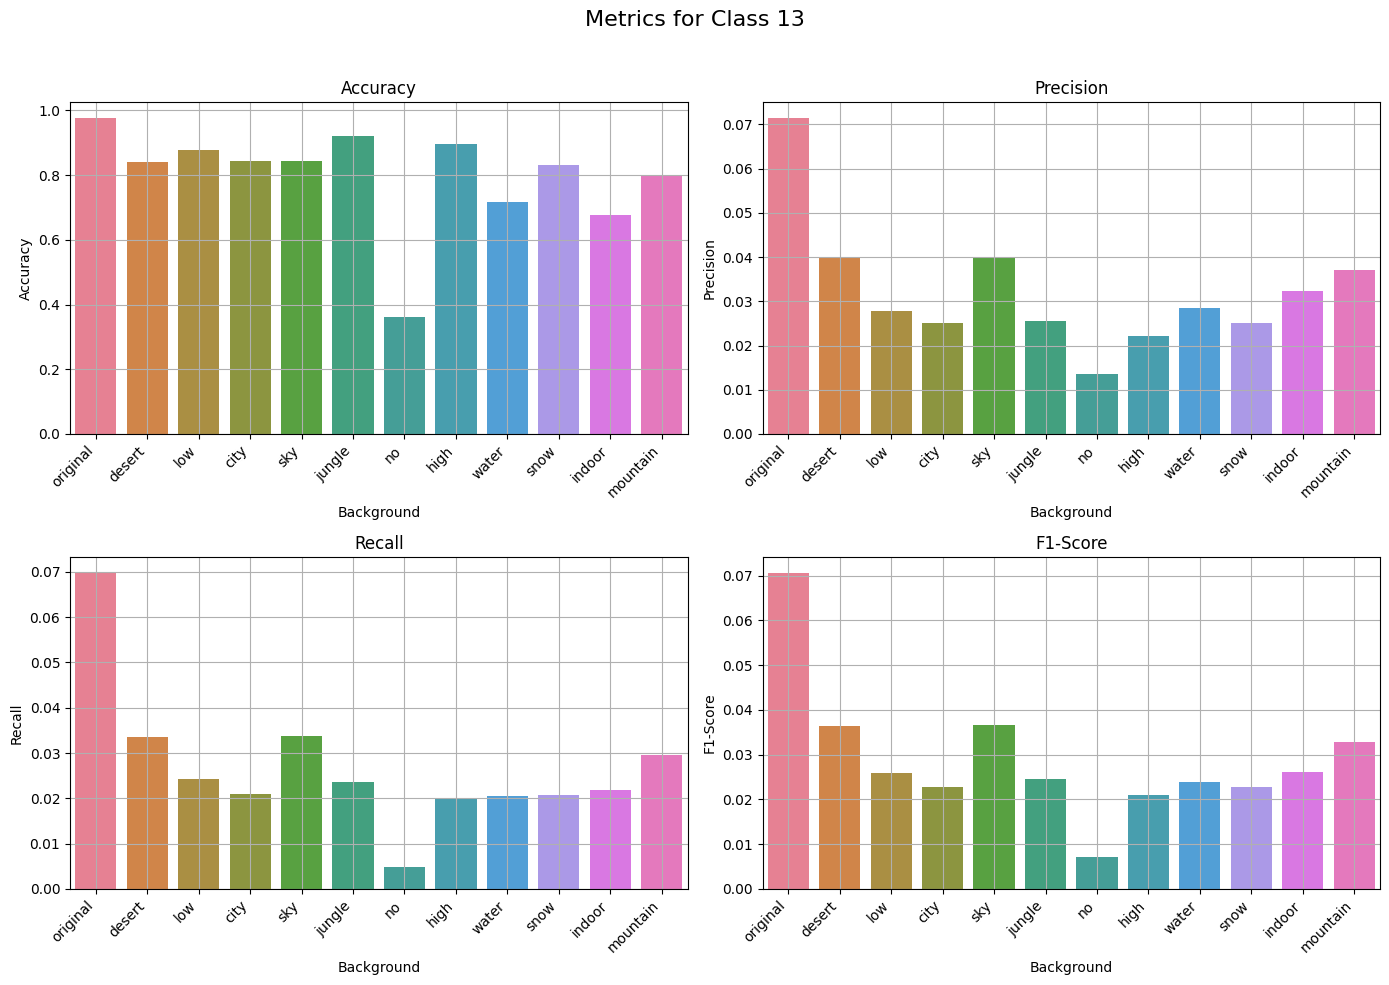
\includegraphics[width=.9\textwidth]{img/13}
	\caption{Metryki}
	\label{rys:13}
\end{figure}

\begin{figure}
	\centering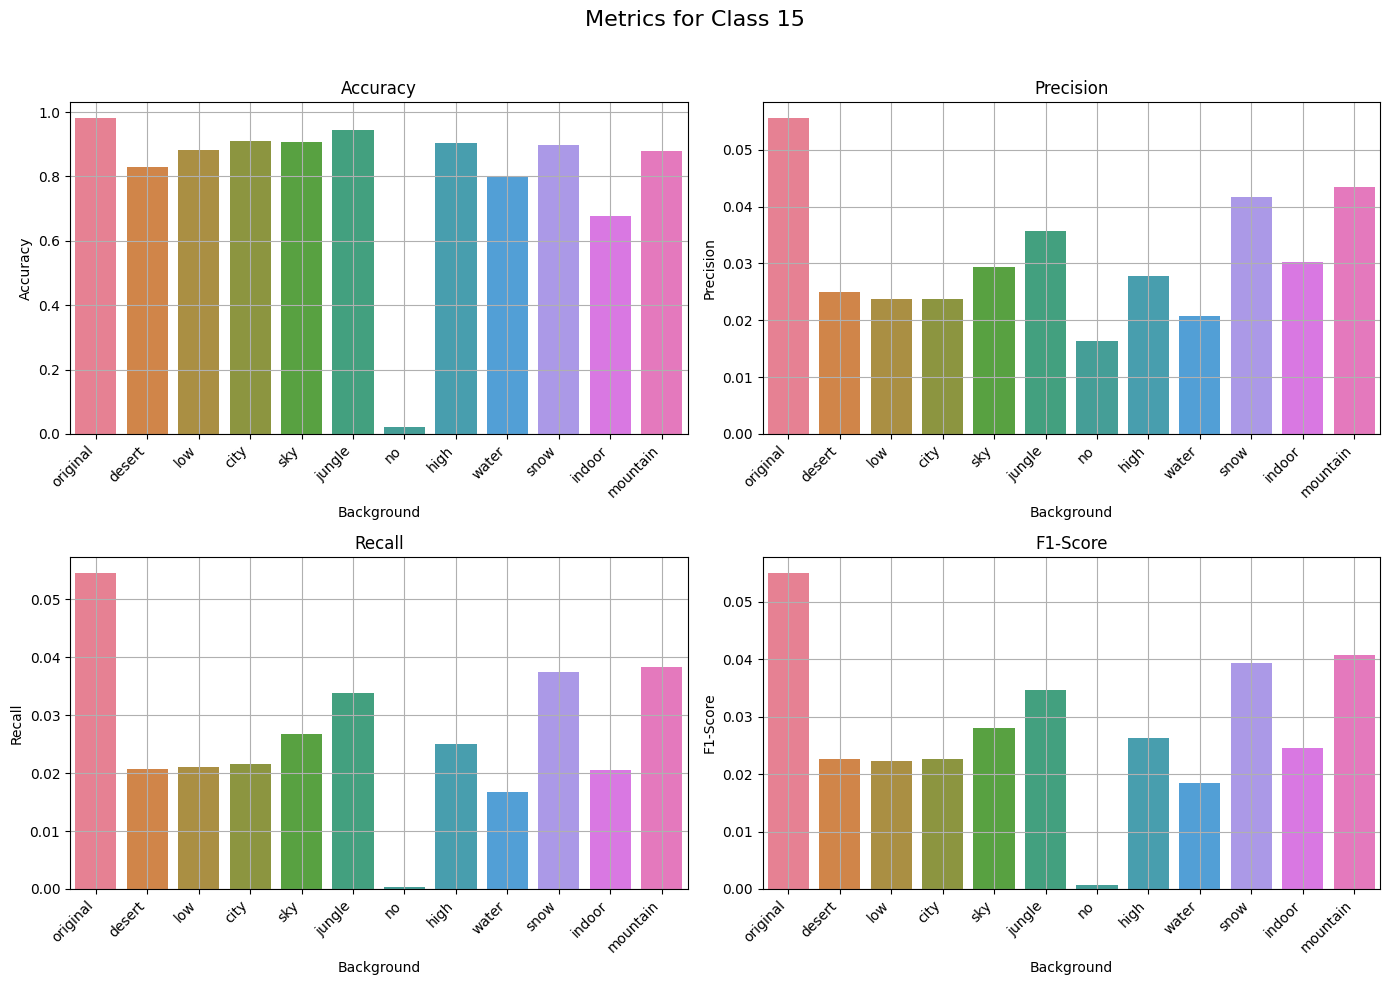
\includegraphics[width=.9\textwidth]{img/15}
	\caption{Metryki}
	\label{rys:15}
\end{figure}

\begin{figure}
	\centering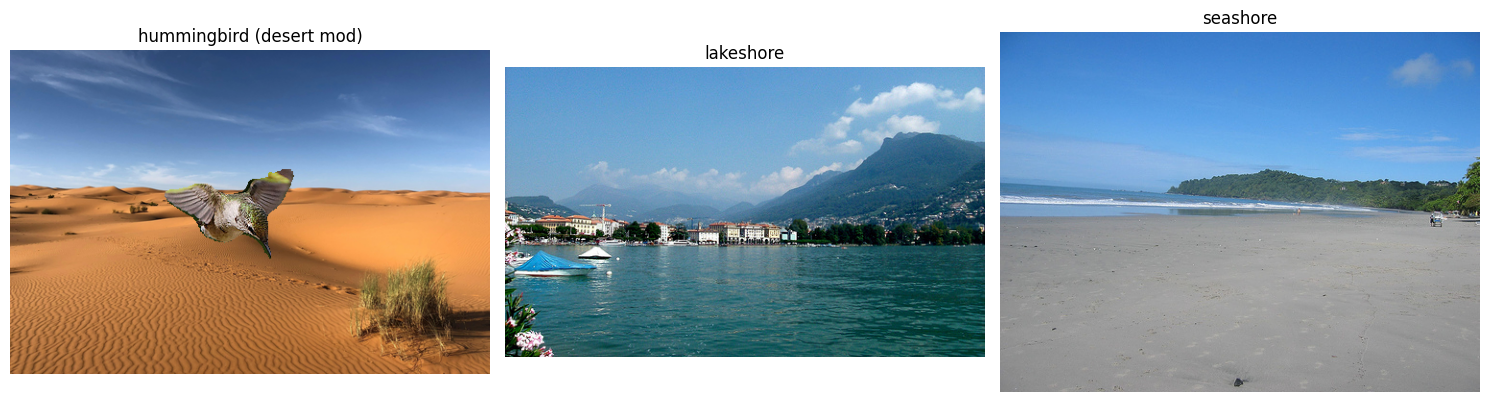
\includegraphics[width=.9\textwidth]{img/94}
	\caption{Metryki}
	\label{rys:94}
\end{figure}

\begin{figure}
	\centering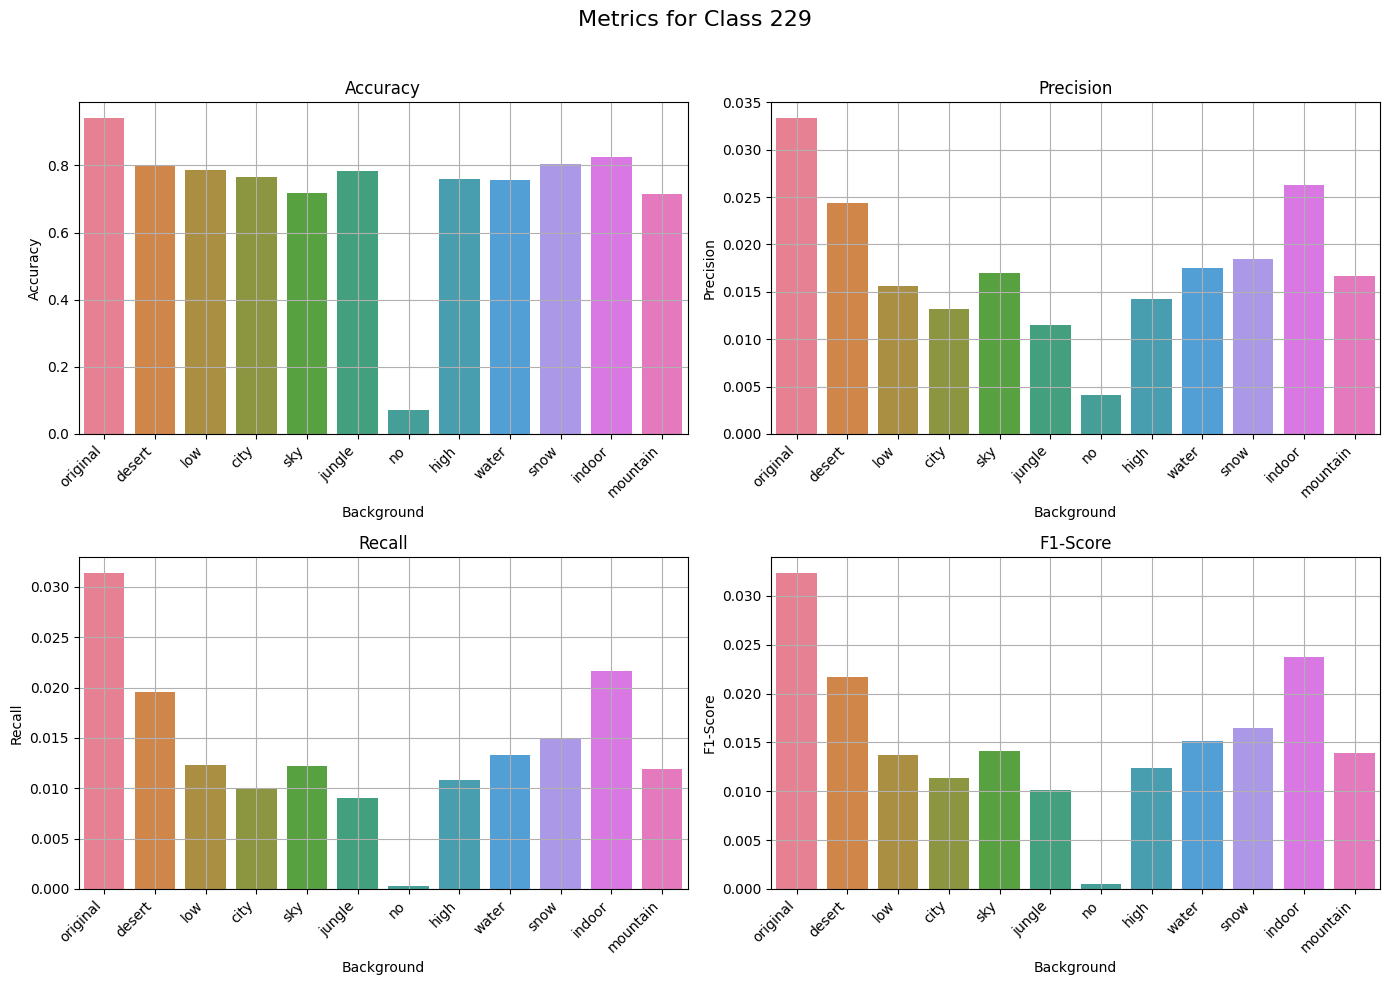
\includegraphics[width=.9\textwidth]{img/229}
	\caption{Metryki}
	\label{rys:229}
\end{figure}

\begin{figure}
	\centering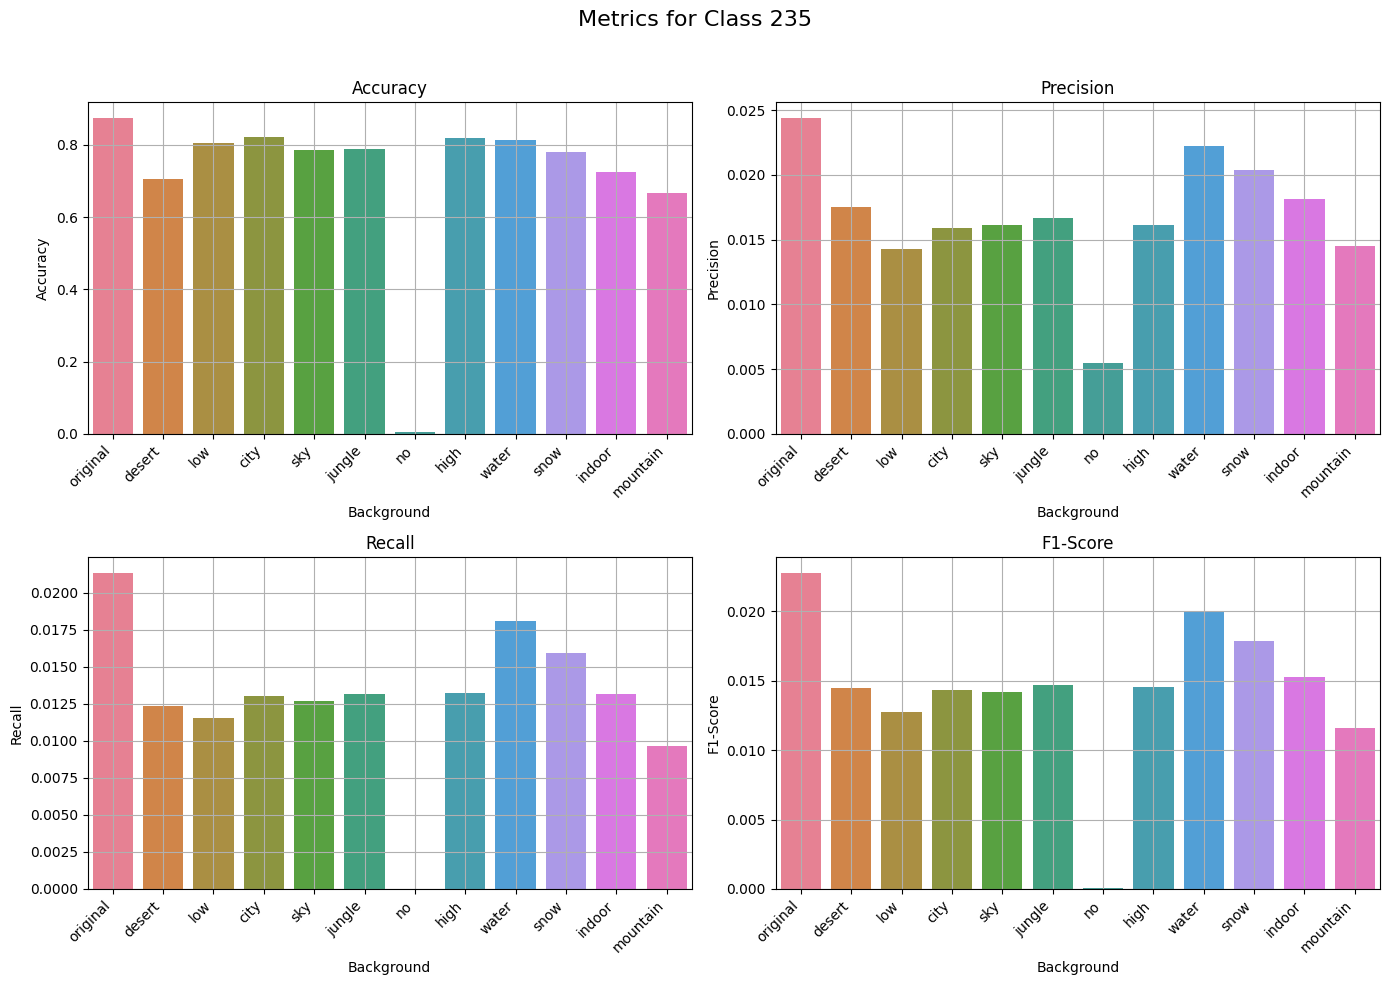
\includegraphics[width=.9\textwidth]{img/235}
	\caption{Metryki}
	\label{rys:235}
\end{figure}

\begin{figure}
	\centering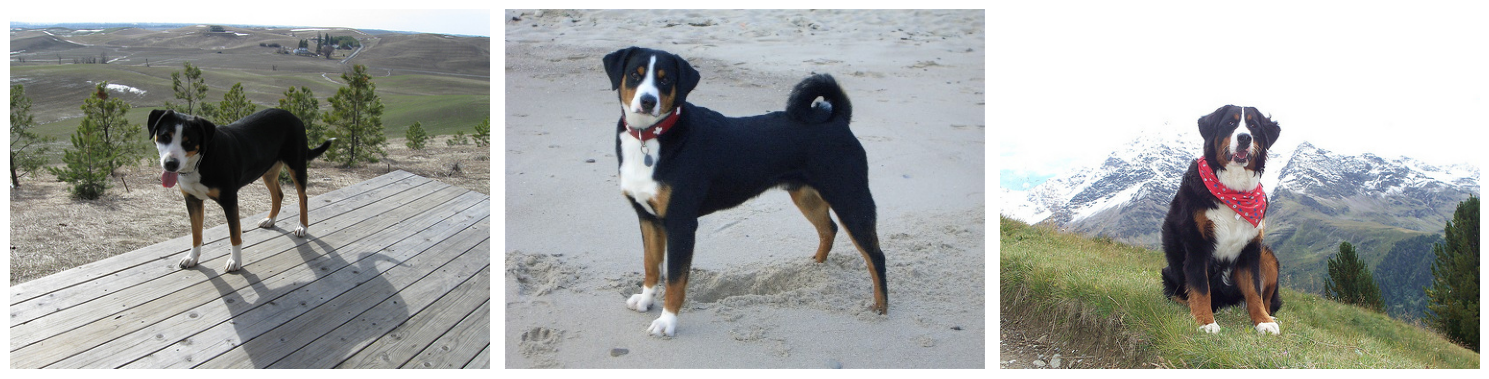
\includegraphics[width=.9\textwidth]{img/238}
	\caption{Metryki}
	\label{rys:238}
\end{figure}

\begin{figure}
	\centering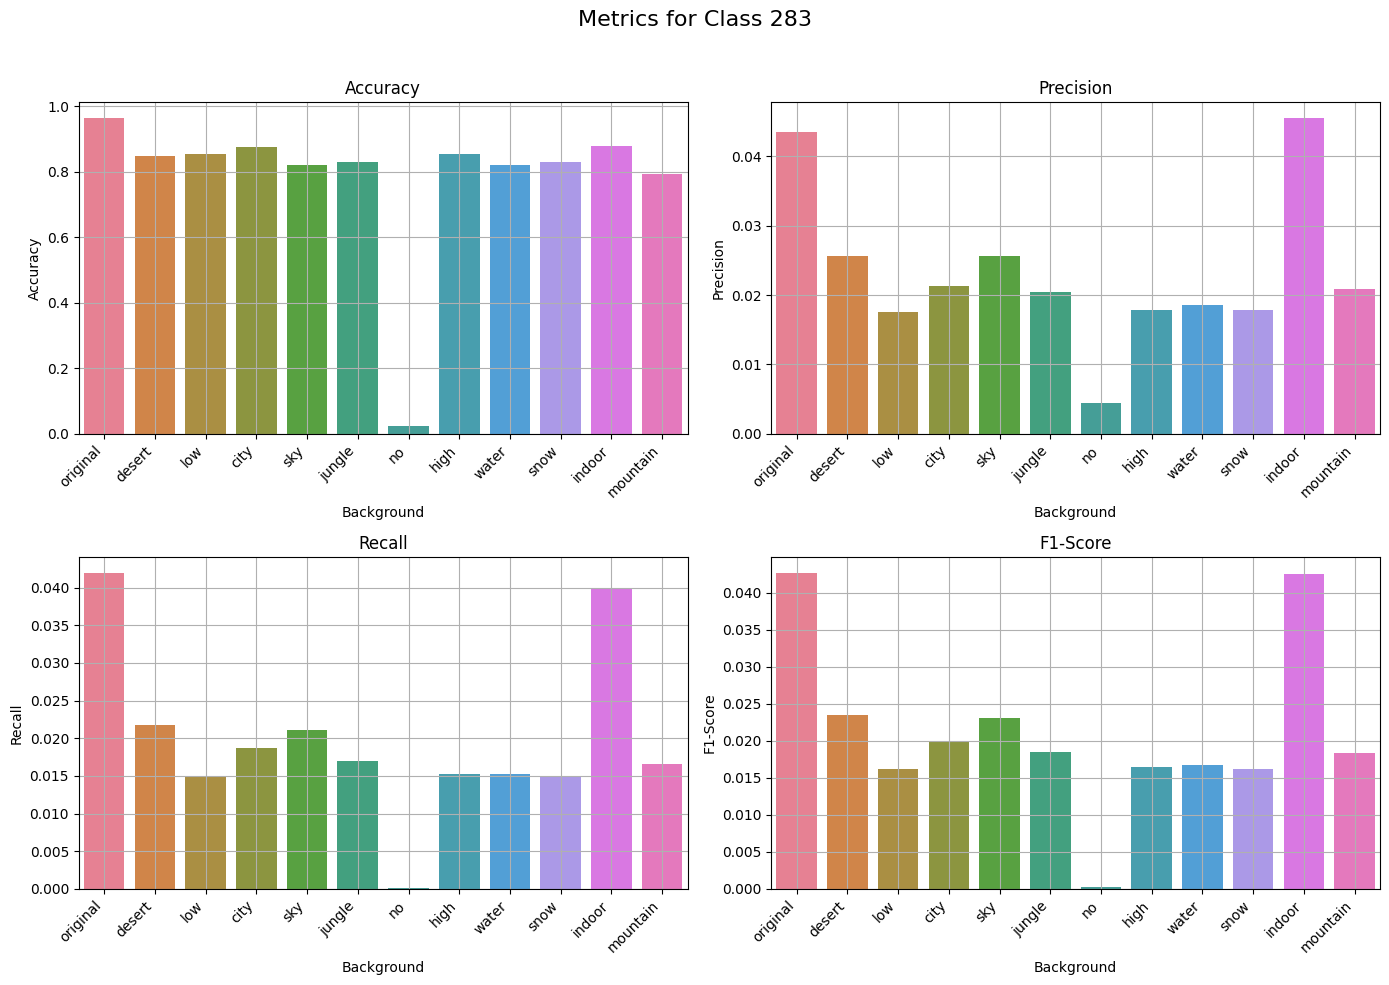
\includegraphics[width=.9\textwidth]{img/283}
	\caption{Metryki}
	\label{rys:283}
\end{figure}

\begin{figure}
	\centering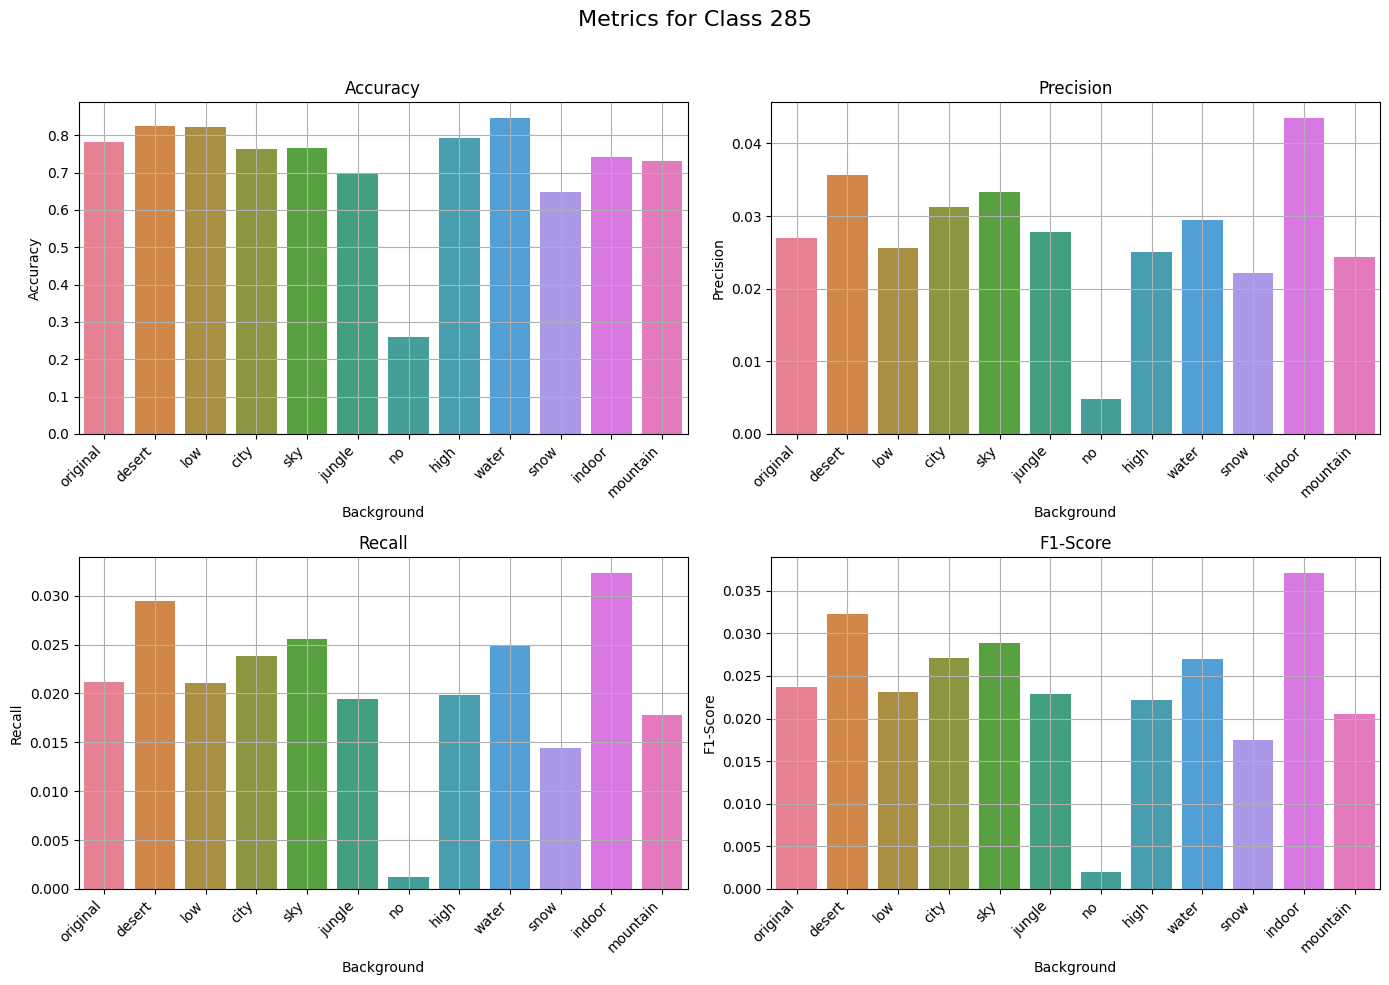
\includegraphics[width=.9\textwidth]{img/285}
	\caption{Metryki}
	\label{rys:285}
\end{figure}

\begin{figure}
	\centering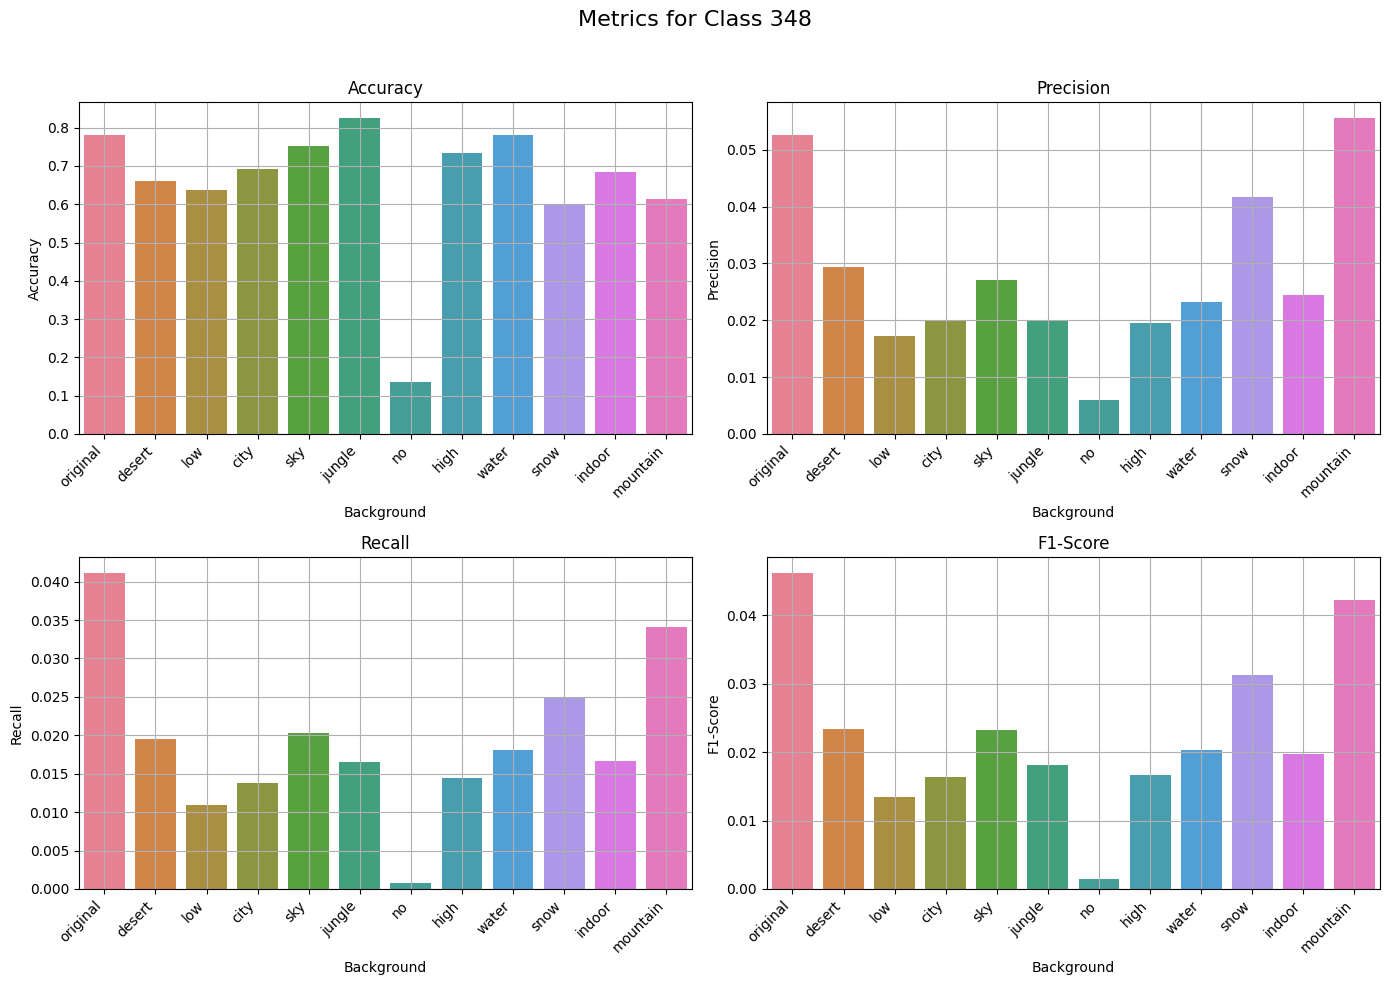
\includegraphics[width=.9\textwidth]{img/348}
	\caption{Metryki}
	\label{rys:348}
\end{figure}

\begin{figure}
	\centering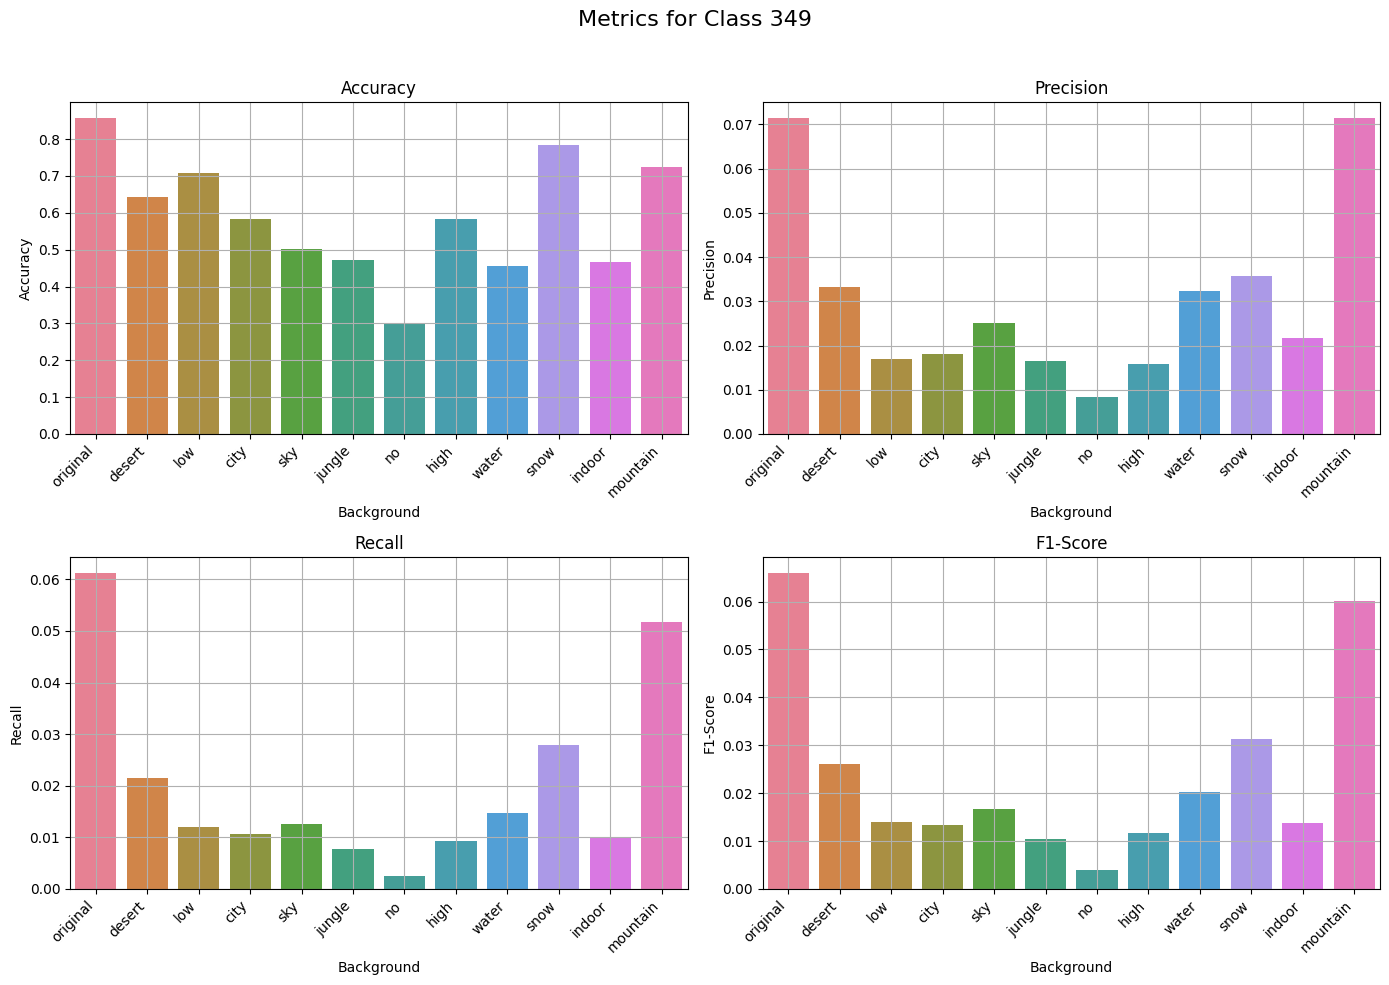
\includegraphics[width=.9\textwidth]{img/349}
	\caption{Metryki}
	\label{rys:349}
\end{figure}

\begin{figure}
	\centering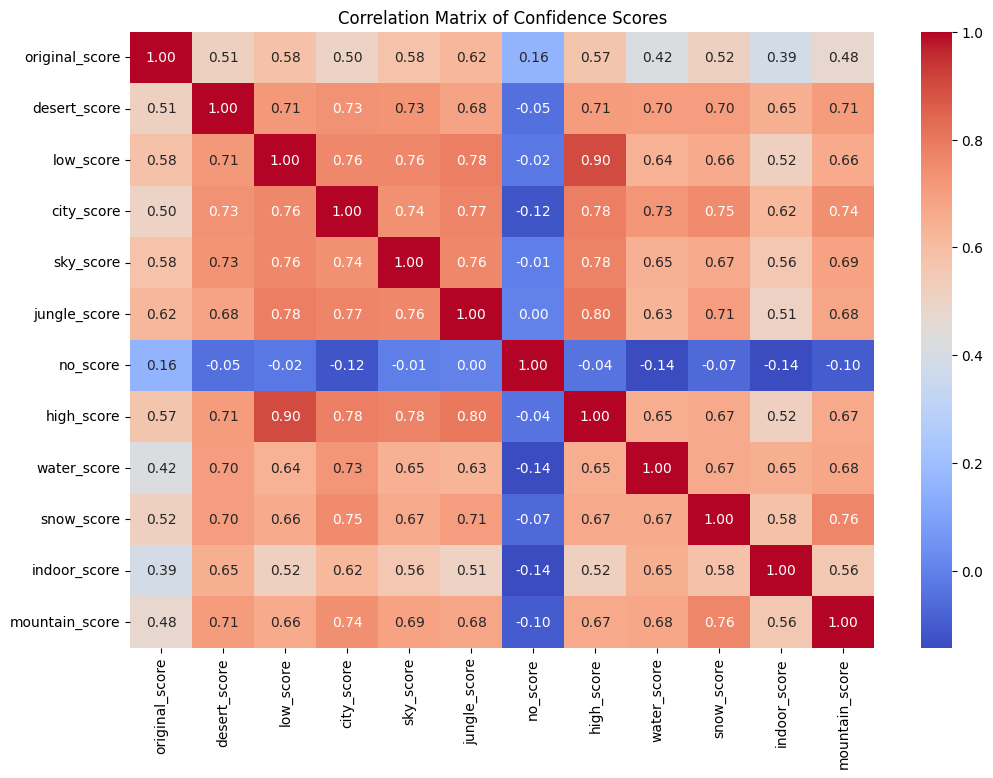
\includegraphics[width=.9\textwidth]{img/correlation_matrix_res}
	\caption{Correlation matrix ResNet confidence}  
    \label{rys:correlation_resnet}
\end{figure}

\begin{figure}
	\centering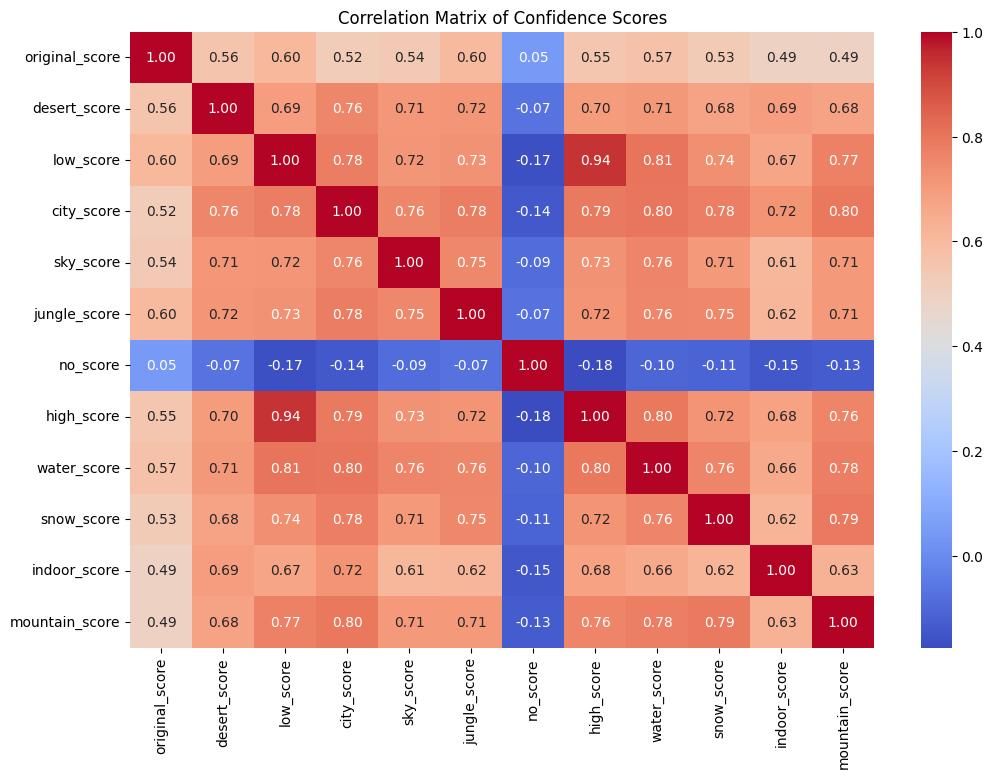
\includegraphics[width=.9\textwidth]{img/correlation_matrix_conv}
	\caption{Correlation matrix ConvNeXt confidence}  
    \label{rys:correlation_convnext}
\end{figure}